\documentclass[a4paper,12pt]{article}
\usepackage[T2A]{fontenc}
\usepackage[utf8]{inputenc}
\usepackage[english,russian]{babel}
\usepackage{listings}
\usepackage{verbatim}
\usepackage{csquotes}
\usepackage{graphicx}
\usepackage[labelsep=period]{caption}
\usepackage{float}
\usepackage[bibencoding=auto,
            backend=biber,
            language=english,
            style=numeric-comp,
            bibstyle=ieee]{biblatex}
\addbibresource{references.bib}

\usepackage{soulutf8}
\usepackage{color}
\sethlcolor{yellow}

\newcommand{\citeisr}{\cite{isrpaper}}
\newcommand{\xvector}{\texttt{x-vector}}
\newcommand{\guesser}{\texttt{Guesser}}
\newcommand{\enquirer}{\texttt{Enquirer}}
\newcommand{\cbenquirer}{\texttt{CodebookEnquirer}}

\author{Головин Вячеслав Сергеевич}
\title{Использование обучения с подкреплением для решения задачи распознавания
диктора в интерактивном режиме}
\date{2023}

\begin{document}

\maketitle

\tableofcontents

\newpage
\section*{Введение}\label{sec:intro}
\addcontentsline{toc}{section}{\protect\numberline{}Введение}

бла-бла-бла, распознавание диктора это важно и полезно\ldots


\section{Распознавание диктора в интерактивном режиме}\label{sec:theory}

\subsection{Задача распознавания диктора}

Распознавание диктора является одной из задач обработки речи --- обширного
научного и исследовательского направления с долгой и богатой историей. Как и в
случае со многими другими научными направлениеями, в последние годы обработка
речи стала активно использовать методы машинного обучения, в частности
нейросетевые модели. \hl{привести примеры моделей?}

Задача распознавания диктора, как нетрудно понять из названия, заключается в
определении личности человека по аудиозаписи его речи. Если говорить чуть
более строго, задачей является сопоставление некоторой аудиозаписи речи
неизвестного человека с некоторым набором дикторов. В случае решения задачи
\emph{идентификации} этот набор состоит из нескольких дикторов, при этом мы
точно знаем, что один из них произнес анализируемую нами речь. Соответственно,
в таком случае задачей системы является правильный выбор диктора. В случае
решения задачи \emph{верификации} нам известна информация только об одном
диктора. Таким образом, от нас требуется определить, произнёс ли он речь на
предоставленной нам аудиозаписи. \hl{криво написано, можно переписать}

\subsection{Интерактивный режим}\label{ssec:isr}

\begin{figure}[htb]
    \centering
    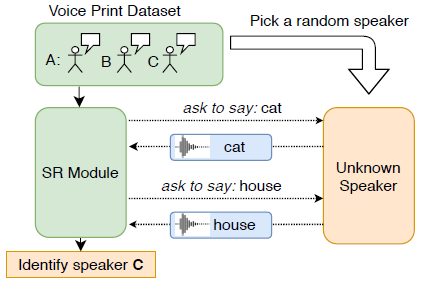
\includegraphics[scale=0.8]{../presentation/figures/isr_game.png}
    \caption{Схема интерактивной игры по определению диктора \citeisr}
\end{figure}

\section{Детали реализации и результаты}\label{sec:experiments}

\subsection{Данные для обучения и извлечение эмбеддингов}

Здесь мы практически полностью повторяем описанный в~\cite{isrpaper} подход.
Единственным (но очень существенным) отличием является использованная размерность
эмбеддингов. Перед тем как перейти к обсуждению этого момента, расскажем про
исходные данные.

Итак, для обучения и тестирования моделей мы использовали датасет
TIMIT\cite{timit}. Он составлен из аудиозаписей речи 630~дикторов, говорящих на
8~основных диалектах американского английского языка. Эти дикторы поделены на
обучающую (\texttt{train}) и тестовую (\texttt{test}) выборки, в первую входят
468~дикторов, во вторую --- 162. Для обучения нейросетевых моделей мы также
создавали валидационную выборку, в которую выделялись 20\% дикторов из обучающей.

Каждый из дикторов произносит 10~фонетически насыщенных предложений. При этом 2
из 10 предложений являются общими для всех дикторов
\footnote{Общие предложения:\\
          \textit{She had your dark suit in greasy wash water all year.}\\
          \textit{Don't ask me to carry an oily rag like that.}}
, остальные 8 уникальны для каждого диктора. Такое разделение позволяет без
особых затруднений подготовить данные, необходимые для описанной
в~\ref{ssec:isr} игры:
\begin{itemize}
    \item 2~общих предложения можно использовать для получения аудиозаписей
    слов.  Для этого разделим аудиозаписи этих предложений по временным
    отметкам, предоставленным создателями датасета. В результате получим 20
    аудиозаписей слов\footnote{Аналогично~\cite{isrpaper} мы не используем слово
    \textit{an}.} для каждого диктора.
    \item 8~уникальных для каждого диктора предложений можно использовать для
    получения голосовых подписей --- эмбеддингов дикторов --- просто при помощи
    усреднения эмбеддингов аудиозаписей этих предложений.
\end{itemize}

В качестве векторов признаков использовались эмбеддинги
\xvector{}~\cite{xvectorspaper}. Весь процесс преобразования аудиозаписей в
векторы признаков осуществлялся с помощью библиотеки Kaldi~\cite{kaldi}. На
первом этапе рассчитывалиcь мел-частотные кепстральные коэффициенты\footnote{
Параметры аналогичны использованным в~\cite{isrpaper} и определяются
требованиями предобученной модели.} и производилось детектирование голосовой
активности (\textit{aнгл.} VAD --- voice activity detection). Полученные векторы
признаков поступали на вход предобученной нейронной сети~\cite{sre16model}. В
качестве эмбеддингов использовались данные со второго 512-мерного слоя.

Здесь, как уже было сказано ранее, мы отступаем от оригинальной работы
\cite{isrpaper}, где использовались 128-мерные эмбеддинги. На это есть две
причины. Во-первых, из приведенных в \cite{isrpaper} комментариев
неочевидно\footnote{
    Цитата: \textit{We then process the MFCCs features through a pretrained
    X-Vector network to obtain a high quality voice embedding of fixed dimension
    128, where the X-Vector network is trained on augmented Switchboard, Mixer~6
    and NIST SREs}.
}, как производилось понижение размерности.
Во-вторых, мотивация такого преобразования тоже неочевидна. Уже первые проведенные
нами эксперименты показали, что при использовании 512-мерных эмбеддингов точность
идентификации оказывается существенно выше приведенных в \cite{isrpaper} значений.

\subsection{Обучение \guesser{}}

\ldots

\subsection{Обучение \enquirer{}}

\ldots

\subsection{Эвристическая модель выбора слов}

\ldots

\section{Модификации метода}\label{sec:modifications}

\subsection{От идентификации к верификации}\label{ssec:verification}

В первых двух главах этого отчёта мы изучали предложенную в~\citeisr{} систему
распознавания диктора. С нашей точки зрения у неё есть серьёзный недостаток ---
она решает задачу \emph{идентификации}, в то время как интересная нам с
практической точки зрения система аутентификации пользователя должна решать
задачу \emph{верификации}. Ранее мы сформулировали тезис о том, что это не
является большой проблемой, и переход идентификация--верификация можно выполнить
без особых проблем. Обсуждению этого вопроса посвящён данный раздел.

Сначала проговорим, как меняется наша задача. Ранее мы должны были выбрать
одного из $K$ дикторов, произнесшего $T$ слов, т.\,е. мы использовали $K$
эмбеддингов дикторов и $T$ эмбеддингов слов. В случае верификации у нас есть
только 1 диктор, от нас требуется ответить на вопрос, является ли он человеком,
произнесшим услышанную нами речь. Подумаем, какие изменения нам нужно внести
в архитектуру использованных нами нейросетей.

В случае \enquirer{} (нейросети для выбора запрашиваемых слов) ответ оказывается
предельно простым --- нам не нужны никакие изменения. Действительно, сами
эмбеддинги диктора на вход этой модели не поступают, используется только их
среднее $\hat{g}$, которое в случае верификации будет просто равно эмбеддингу
единственного диктора.

\begin{table}[htb]
    \centering
    \begin{tabular}{c c c}
        \toprule
        Выбор слов & Режим обучения & Точность\\
        \midrule
        случайный & \multirow{3}{4em}{$T = 3$} & 0.895 \\
        \enquirer{} & & 0.933\\
        эвристика & & 0.917\\
        \midrule
        случайный & \multirow{3}{4em}{$T = 2$} & 0.913 \\
        \enquirer{} & & 0.947\\
        эвристика & & 0.945\\
        \bottomrule
    \end{tabular}
    \caption{Точность верификации, $T = 3$ запрашиваемых слова}
    \label{tab:ver}
\end{table}

Ситуация с \guesser{} лишь немного сложнее. Т.\,к. его архитектура позволяет
рассматривать игры с произвольным числом дикторов, проблемы возникают только на
самом последнем слое, выполняющим операцию $\softmax$. На данном этапе у
модели (для каждой игры) есть только одно число, которое фактические является
некоторой метрикой соответствия между взвешенной суммой эмбеддингов слов
$\hat{x}$ и эмбеддингом диктора $g$. В таком случае для принятия решения о
(не-)соответствии речи и диктора логично применить операцию $\sigmoid$
(логистическую функцию), превращающее эту метрику в число от $0$ до $1$.

Действительно, такое простое преобразование позволяет получить работающую
систему верификации диктора. Полученные результаты приведены в
табл.~\ref{tab:ver}. Как и в случае идентификации, обучение в более тяжелом
режиме (здесь мы можем только сокращать число запрашиваемых слов) позволяет
немного улучшить результаты, но при этом преимущество перед простым эвристическим
агентом\footnote{
    Градация слов при переходе к верификации практически не меняется.
} тоже является минимальным.

\subsection{\cbenquirer{} --- гибкая система выбора слов}\label{ssec:codebook}

Перейдём к обсуждению другой проблемы оригинальной модели --- наличия
фиксированного списка слов. Действительно, в качестве одного из преимуществ
разрабатываемой системы мы ранее называли возможность делать разнообразные
запросы. Однако используемый до данного момента времени вариант \enquirer{}
слабо соответствует этому требованию --- он осуществляет выбор из 20 слов.
Конечно, этот список может быть и больше, просто для этого потребуется больший
объём данных для обучения. Но при добавлении любого слова будет необходимо либо
заново обучать \enquirer{}, либо выполнять fine-tuning, что выглядит не самым
оптимальным вариантом для готового продукта.

Для решения этой проблемы была разработана архитектура \cbenquirer{}. Она
представляет собой простую модификацию оригинальной модели:
\begin{enumerate}
    \item ``Голова'' модели представляет собой \enquirer{}, в котором число
    выходов равно размерности эмбеддингов, и к ним не применяется операция
    $\softmax$. Таким нехитрым способом мы преобразовали выходы модели из
    вероятностного распределения по словарю в эмбеддинг запрашиваемого слова.
    \item Естественно, стоящая перед \cbenquirer{} задача никак не поменялась ---
    у нас все ещё существует некоторый конечный набор слов, из которых на
    каждом шаге игры нам нужно выбрать одно (или, что лучше, получить
    распределение). Для этого мы составляем \texttt{Codebook} --- тензор из
    эмбеддингов слов, которые рассчитываются как среднее по всем дикторам из
    обучающей выборки.
    \item Наконец, нам нужно как-то сопоставить возвращаемый моделью эмбеддинг
    с эмбеддингами из \texttt{Codebook}. Самый очевидный вариант --- просто
    найти ближайший по $L_2$-норме. Примерно это мы и делаем, вероятность
    выбрать $i$-ое слово из \texttt{Codebook} вычисляется по формуле:
    \begin{equation*}
        p_i = \frac{\exp{(-d_i/T)}}{\sum_{j=0}^{V}{\exp{(-d_j/T)}}},
    \end{equation*}
    где $d_i$ --- расстояние\footnote{
        Для численной стабильности мы используем среднеквадратичную ошибку (MSE)
        вместо $L_2$-нормы.
    } между выходным эмбеддингом и $i$-ым вектором из \texttt{Codebook}, $T$ ---
    обучаемый параметр модели, $V$ --- размер словаря.
\end{enumerate}

В наших экспериментах такая модификация показала практически такие же
результаты, что и оригинальная версия \enquirer{}. Далее мы решили
проверить, возможно ли изменение набора слов без дообучения модели. Для этого
мы обучили \cbenquirer{} на половине словаря и протестировали его на другой
половине. В таком случае мы наблюдали лишь небольшое падение точности\footnote{
    Например, точность обученной в режиме $K = 20$, $T = 2$ модели упала с
    98.9\% до 98.0\%.
}, которое,
скорее всего, просто объясняется уменьшением размера используемого словаря.

\subsection{Добавление шума}

Следующим экспериментом была проверка того, будет ли работать предложенный
подход при наличии фонового шума. Для этого мы выбрали 6~аудиозаписей шума
из датасета MUSAN~\cite{musan2015} и добавили их случайные фрагменты\footnote{
    Аудиозаписи специально выбирались таким образом, чтобы их случайные
    короткие фрагменты отличались слабо.
} к аудиозаписям слов. Соотношение сигнал~/~шум было выбрано равным 3~дБ.
При обучении и тестировании моделей тип шума выбирался случайно, но он не
менялся в течение игры.

\begin{table}[htb]
    \centering
    \begin{tabular}{c c c}
        \toprule
        Выбор слов & Идентификация & Верификация\\
        \midrule
        случайный & 0.887 & 0.895\\
        \enquirer{} & 0.946 & 0.934\\
        эвристика & 0.957 & 0.938\\
        \bottomrule
    \end{tabular}
    \caption{Точность идентификации и верификации в стандартных режимах
    ($T = 3$ слова, $K = 5$ гостей при идентификации) при добавлении фонового
    шума.}
    \label{tab:noise}
\end{table}

Полученные результаты приведены в табл.~\ref{tab:noise}. Видно, что добавление
шума сделало задачу тяжелее, из-за чего точность SR-систем немного упала. Также
любопытно, что простой эвристический агент снова не проиграл \enquirer{} и даже
оказался немного (на уровне погрешности) лучше. Причина этого стала понятна
после измерения средней точности \guesser{} на аудиозаписях зашумлённых слов:
выяснилось, что хотя добавление того или иного типа шума влияет на градацию слов
(которую использует эвристический агент), этот эффект невелик. Иными словами,
``хорошие'' слова, с помощью которых в среднем достигается самая высокая
точность распознавания диктора, остались такими же и при добавлении различных
типов фонового шума.

\subsection{Альтернативные эмбеддинги}\label{ssec:cpc}

Во всех описанных ранее экспериментах для получения эмбеддингов мы использовали
\xvector{}~\cite{xvectorspaper}, повторяя подход авторов оригинальной статьи.
Проблема в том, что выбор таких старых (2017~год) эмбеддингов выглядел немного
странным уже на момент написания оригинальной статьи (2020~год).% Сегодня же они
% выглядят безнадёжно устаревшими.

Поэтому для последнего эксперимента мы проверили, как разработанная SR-модель
работает с другими эмбеддингами. Для этого использовалась нейросеть, обученная
нашими коллегами из лаборатории Huawei CBG AI на 960~часах аудиозаписей из
датасета LibriSpeech\cite{librispeech} и использующая метод контрастного
прогнозирующего кодирования\cite{oord2019representation}.

\begin{table}[htb]
    \centering
    \begin{tabular}{c c c}
        \toprule
        Выбор слов & \xvector{} & CPC\\
        \midrule
        случайный & 0.755 & 0.946\\
        \enquirer{} & 0.914 & 0.990\\
        \bottomrule
    \end{tabular}
    \caption{Точность идентификации при использовании различных типов
    эмбеддингов. $K = 20$, $T = 2$.}
    \label{tab:cpc}
\end{table}

Пример результатов показан в табл.~\ref{tab:cpc}. Общий вывод прост --- замена
эмбеддингов позволяет существенно повысить точность, как при случайном выборе
слов, так и при использовании \enquirer{}.

\subsection{Выводы и результаты по главе}

\begin{itemize}
    \item Мы адаптировали разработанную модель под практическую задачу ---
    перешли от идентификации к верификации, сделали возможной быструю замену
    используемых слов. Внесенные модификации не приводят к существенному понижению
    точности распознавания.
    \item Разработанная модель работает и в присутствие шума на поступающих
    аудиозаписях (по крайней мере, если она была обучена на аугментированных
    данных). При этом преимущество \enquirer{} над эвристическим агентом не
    возрастает.
    \item Использование альтернативных эмбеддингов может существенно изменить
    точность системы.
\end{itemize}

\section*{Заключение}
\addcontentsline{toc}{section}{\protect\numberline{}Заключение}

все работает, но хотелось бы большего

\printbibliography[title=Список литературы]

\end{document} % Конец текста.